\documentclass[../main/main.tex]{subfiles}

\begin{document}
\espacio

  %------------ TODO ------------%
  En este capítulo se muestra el marco teórico TODO.

  \section{Antecedentes}

  \subsection{Computación paralela}

  La computación paralela es una rama de la informática que se encarga del estudio de la ejecución de una tarea dividida en sub-procesos o varias tareas independientes de forma simultánea en forma de hilos de ejecución en un grupo de procesadores llamados también procesadores multinúcleo, que luego de realizar dichas tareas sincronizan sus resultados a fin de mantener la integridad de los datos.

  \begin{figure}[H]
    \centering
    \caption{Disposición de un microprocesadores multinúcleo}
    \begin{center}
\end{center}


\tikzset{every picture/.style={line width=0.75pt}} %set default line width to 0.75pt        

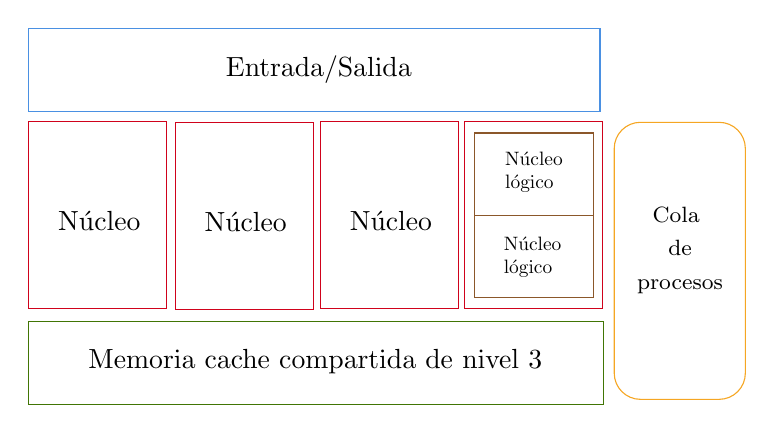
\begin{tikzpicture}[x=0.75pt,y=0.75pt,yscale=-1,xscale=1]
%uncomment if require: \path (0,300); %set diagram left start at 0, and has height of 300

%Shape: Rectangle [id:dp7451660985771589] 
\draw  [color={rgb, 255:red, 208; green, 2; blue, 27 }  ,draw opacity=1 ] (101.31,109) -- (167.81,109) -- (167.81,199.2) -- (101.31,199.2) -- cycle ;

%Shape: Rectangle [id:dp20887119442499946] 
\draw  [color={rgb, 255:red, 208; green, 2; blue, 27 }  ,draw opacity=1 ] (171.81,109.5) -- (238.31,109.5) -- (238.31,199.7) -- (171.81,199.7) -- cycle ;

%Shape: Rectangle [id:dp7286280016278224] 
\draw  [color={rgb, 255:red, 208; green, 2; blue, 27 }  ,draw opacity=1 ] (241.81,109) -- (308.31,109) -- (308.31,199.2) -- (241.81,199.2) -- cycle ;

%Shape: Rectangle [id:dp10536868660856769] 
\draw  [color={rgb, 255:red, 208; green, 2; blue, 27 }  ,draw opacity=1 ] (311.31,109) -- (377.81,109) -- (377.81,199.2) -- (311.31,199.2) -- cycle ;
%Shape: Rectangle [id:dp1826752439641639] 
\draw  [color={rgb, 255:red, 65; green, 117; blue, 5 }  ,draw opacity=1 ] (101.17,205.17) -- (378.06,205.17) -- (378.06,245.17) -- (101.17,245.17) -- cycle ;
%Rounded Rect [id:dp2234320479476144] 
\draw  [color={rgb, 255:red, 245; green, 166; blue, 35 }  ,draw opacity=1 ] (383.33,121.97) .. controls (383.33,114.99) and (388.99,109.33) .. (395.97,109.33) -- (433.87,109.33) .. controls (440.84,109.33) and (446.5,114.99) .. (446.5,121.97) -- (446.5,230.17) .. controls (446.5,237.14) and (440.84,242.8) .. (433.87,242.8) -- (395.97,242.8) .. controls (388.99,242.8) and (383.33,237.14) .. (383.33,230.17) -- cycle ;
%Shape: Rectangle [id:dp1417047542970684] 
\draw  [color={rgb, 255:red, 74; green, 144; blue, 226 }  ,draw opacity=1 ] (101,64) -- (376.5,64) -- (376.5,104) -- (101,104) -- cycle ;
%Shape: Rectangle [id:dp36104680527645483] 
\draw  [color={rgb, 255:red, 139; green, 87; blue, 42 }  ,draw opacity=1 ] (316,114.5) -- (373.25,114.5) -- (373.25,154.1) -- (316,154.1) -- cycle ;
%Shape: Rectangle [id:dp8737201655413631] 
\draw  [color={rgb, 255:red, 139; green, 87; blue, 42 }  ,draw opacity=1 ] (316,154.1) -- (373.25,154.1) -- (373.25,193.7) -- (316,193.7) -- cycle ;

% Text Node
\draw (135.25,157) node  [align=left] {Núcleo};
% Text Node
\draw (205.75,157.5) node  [align=left] {Núcleo};
% Text Node
\draw (275.75,157) node  [align=left] {Núcleo};
% Text Node
\draw (239.33,224.67) node  [align=left] {Memoria cache compartida de nivel 3};
% Text Node
\draw (415,171) node  [align=left] {{\footnotesize  \ \ Cola}\\{\footnotesize  \ \ \ \ de}\\{\footnotesize procesos}};
% Text Node
\draw (241,84) node  [align=left] {Entrada/Salida};
% Text Node
\draw (344.67,133.33) node [scale=0.7] [align=left] {Núcleo\\ lógico};
% Text Node
\draw (344,174.33) node [scale=0.7] [align=left] {Núcleo\\ lógico};


\end{tikzpicture}
\begin{center}
\end{center}

    \caption*{\textbf{Fuente:} Elaboración propia}
  \end{figure}

  Los microprocesadores actuales contienen comúnmente dos tipos de núcleos, los núcleos físicos y los núcleos lógicos. Cada zócalo de una tarjeta madre contiene un microprocesador, este contiene uno o más núcleos físicos; un núcleo físico es aquel que se encuentra físicamente dentro del circuito integrado del microprocesador, mientras que un núcleo lógico es una división virtual en 2 o más partes de un núcleo físico. Las tareas son asignadas a los núcleos físicos; estas tareas pueden dividirse en tareas más pequeñas a fin de resolver un gran problema en partes pequeñas que al final serán unidas para generar la solución, estas partes pequeñas son llamadas ``hilos'' y son las que se ejecutan en los núcleo lógicos.

  \textit{Las técnicas principales para lograr estas mejoras de rendimiento (mayor frecuencia de reloj y arquitecturas cada vez más inteligentes y complejas) están golpeando la llamada ``Power Wall''. La industria informática ha aceptado que los futuros aumentos en rendimiento deben provenir en gran parte del incremento del número de procesadores (o núcleos) en una matriz, en vez de hacer más rápido un solo núcleo.} [\cite[p.~6]{report:parallel_computing_illinois}]

  El incremento de la frecuencia en los microprocesador acarrea consigo el consumo de energía y la disminución del espacio entre los transistores dentro de cada núcleo, lo que provoca un incremento considerable de la temperatura dentro del microprocesador; por tanto, para mantener el microprocesador en funcionamiento evitando su deterioro por las temperaturas elevadas es necesario buscar fuentes más óptimas de enfriado como los tubos de conducción de gas o líquido, que incrementan aún más el consumo de energía y que son costosos para una PC de escritorio.

  \begin{equation}
    T_m = T_a \cdot [( 1 - F_m ) + \frac{F_m}{A_m}]
    \label{ecuacion_amdahl}
  \end{equation}

  Donde:

  \begin{description}[noitemsep, nolistsep]
    \item[$F_m=$] Fracción de tiempo que el sistema utiliza el subsistema mejorado
    \item[$A_m=$] Factor de mejora que se ha introducido en el subsistema mejorado
    \item[$T_a=$] Tiempo de ejecución antiguo
    \item[$T_m=$] Tiempo de ejecución mejorado
  \end{description}

  Por tales motivos Gene Amdahl formuló la ecuación \ref{ecuacion_amdahl} que establece que:

  \textit{La mejora obtenida en el rendimiento de un sistema debido a la alteración de uno de sus componentes está limitada por la fracción de tiempo que se utiliza dicho componente}

  Despejando la ecuación \ref{ecuacion_amdahl} se obtiene la aceleración del programa completo una vez que se haya paralelizado uno o más algoritmos del programa.

  \begin{equation}
    A = \frac{1}{( 1 - F_m ) + \frac{F_m}{A_m}}
    \label{ecuacion_amdahl_aceleracion}
  \end{equation}

  Donde:

  \begin{description}[noitemsep, nolistsep]
    \item[$A=$] Aceleración o ganancia en velocidad conseguida en el sistema completo debido a la mejora de uno de sus subsistemas
    \item[$A_m=$] Factor de mejora que se ha introducido en el subsistema mejorado
    \item[$F_m=$] Fracción de tiempo que el sistema utiliza el subsistema mejorado
  \end{description}

  \begin{figure}[H]
    \centering
    \caption{Clúster de alto rendimiento}
    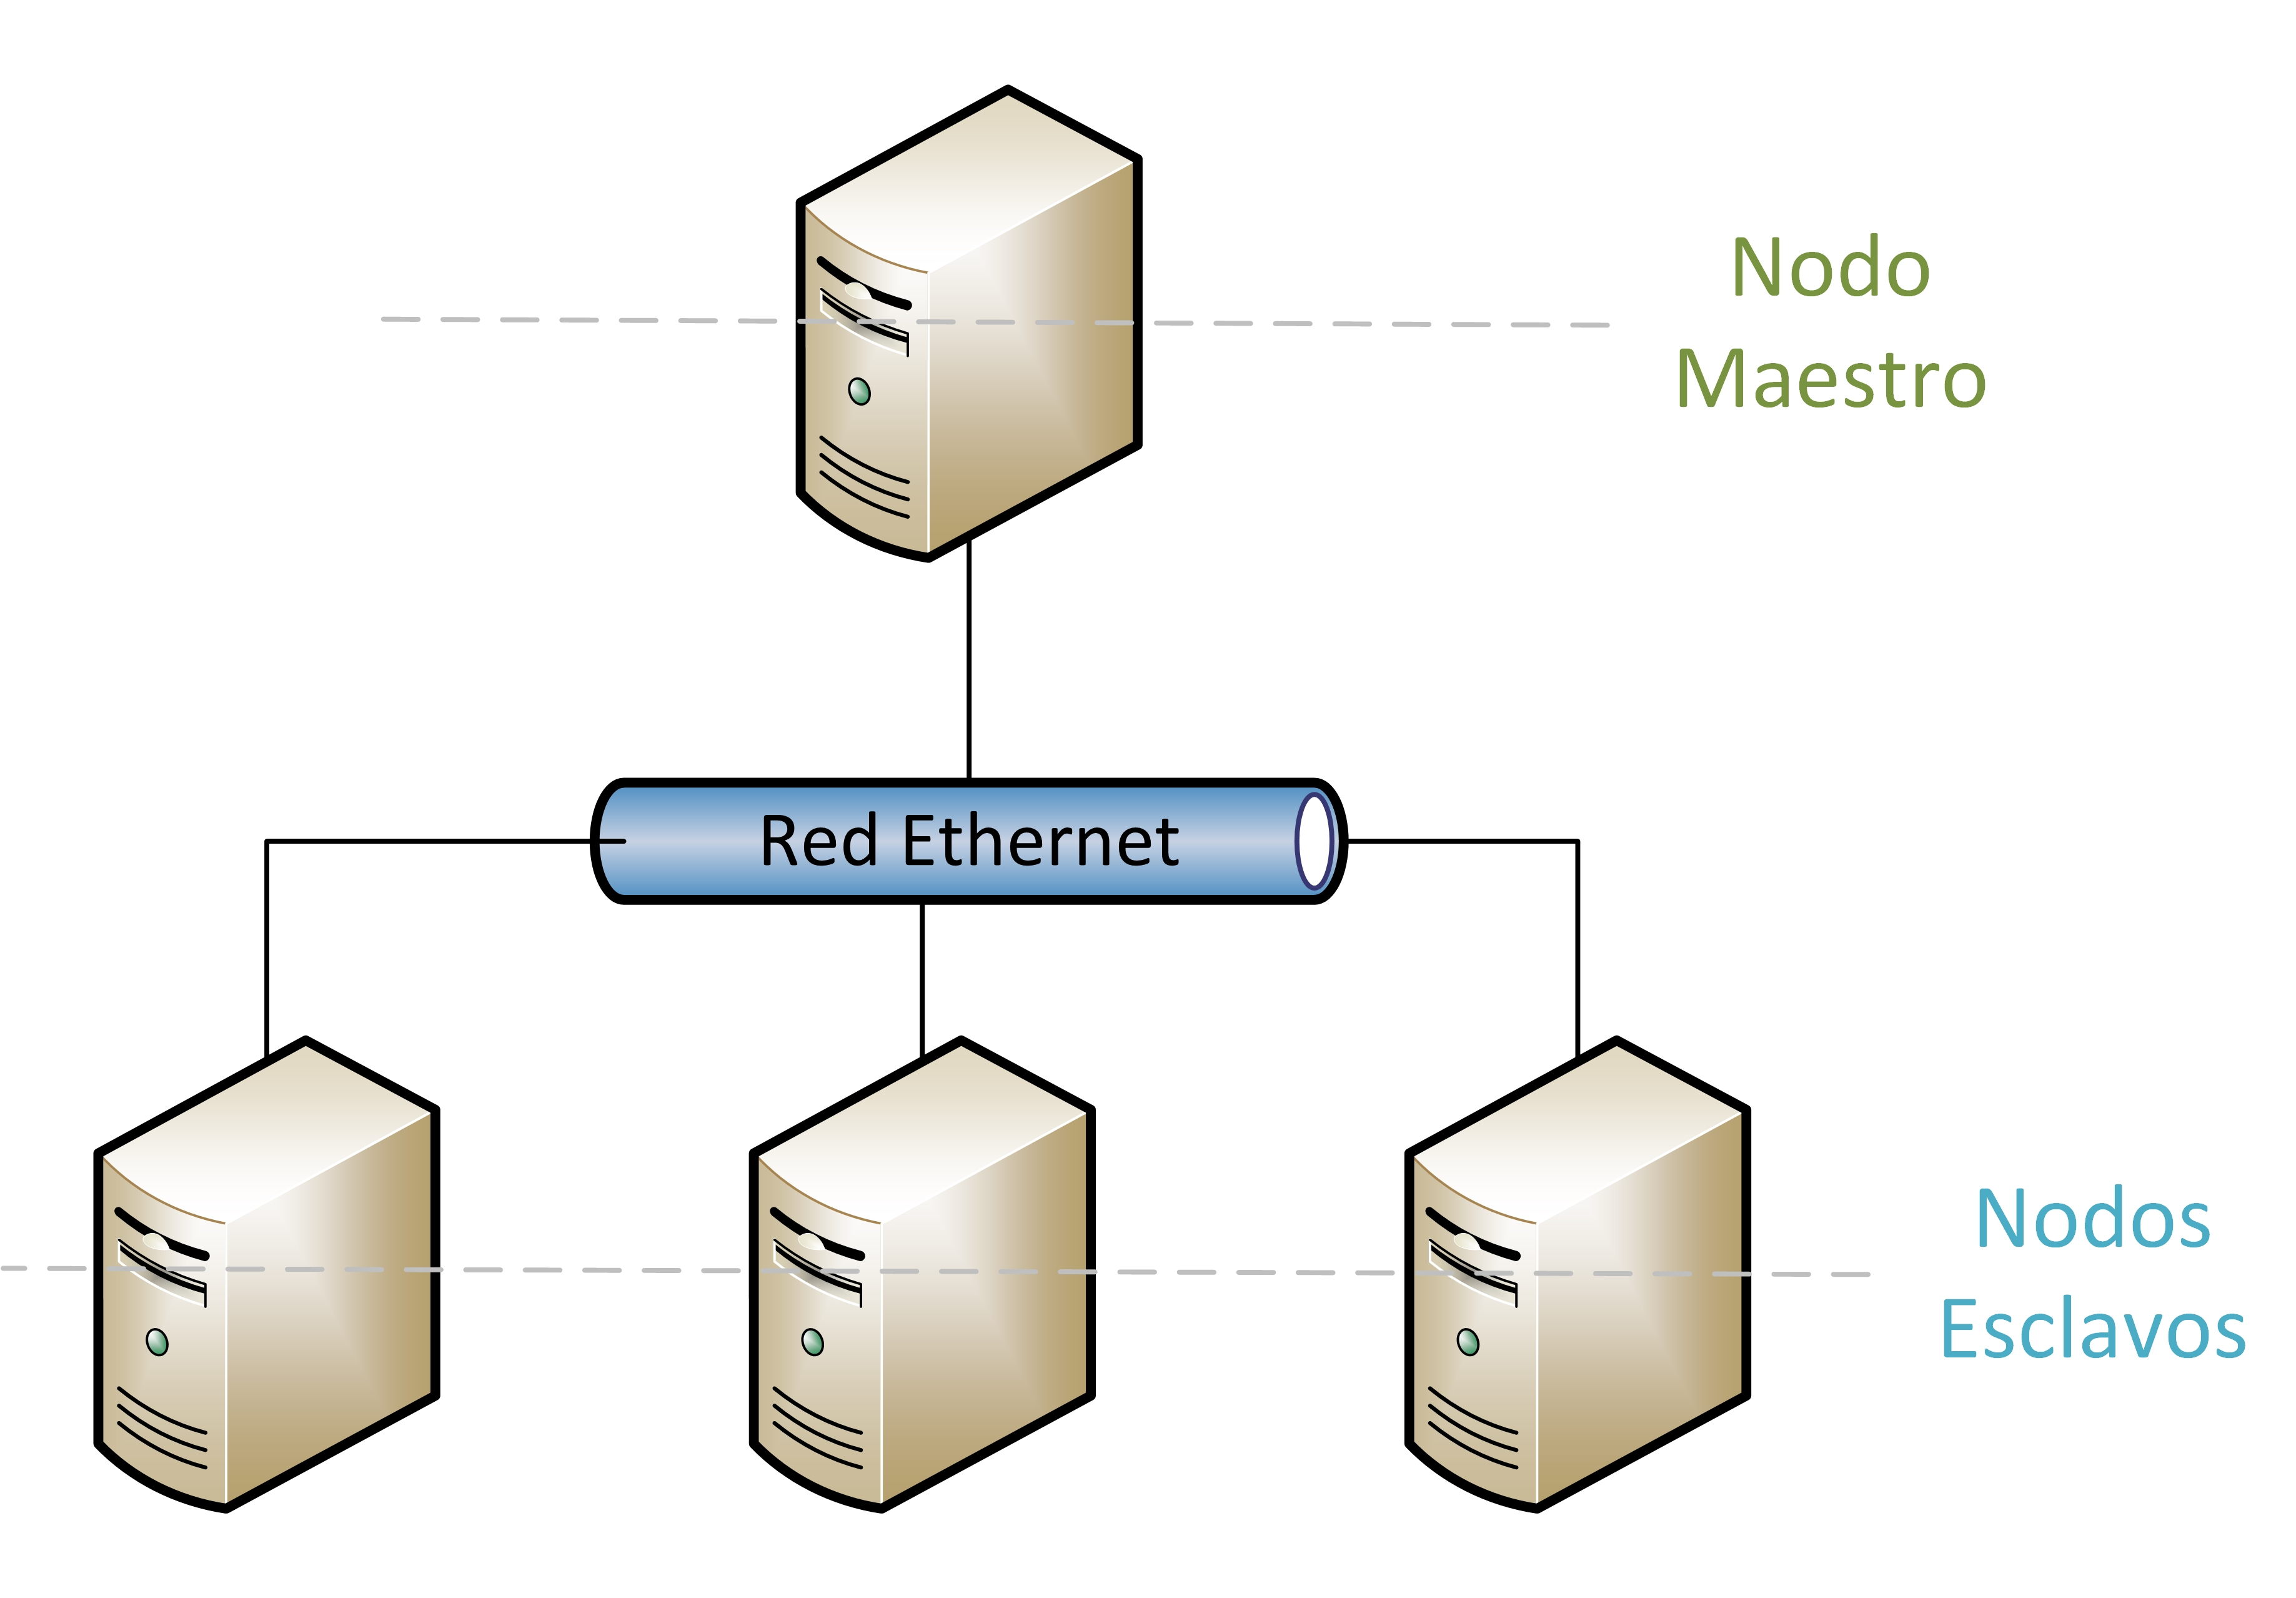
\includegraphics[width=10cm, keepaspectratio]{marco_teorico/cluster_alto_rendimiento.jpg}
    \caption*{\textbf{Fuente:} \cite[p.~2]{article:cluster_alto_rendimiento}}
  \end{figure}

  En base a este principio se desarrollaron tecnologías de matrices de núcleos de cómputo tomando como elementos principales a los procesadores existentes y acomodándolos de tal forma que se pueda administrar la ejecución de tareas en cada procesador de manera individual y la sincronización de resultados al final del proceso. Estos arreglos reciben el nombre de clústers. Los clústers de alto rendimiento son un tipo de clústers utilizados con el propósito de ejecutar tareas exhaustivas divididas en tareas pequeñas ejecutadas en cada computador de acuerdo a la gestión realizada por el llamado nodo maestro. [\cite{article:cluster_alto_rendimiento}]

  \begin{figure}[H]
    \centering
    \caption{Comparación de tiempos de proceso en múltiples CPUs}
    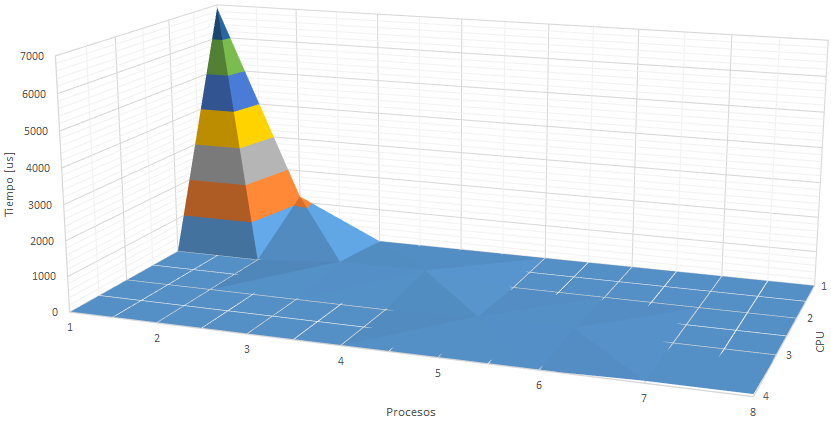
\includegraphics[width=15cm, keepaspectratio]{marco_teorico/resultado_cpu_cluster.png}
    \caption*{\textbf{Fuente:} \cite[p.~7]{article:cluster_alto_rendimiento}}
  \end{figure}

  \section{Unidad de procesamiento gráfico (GPU)}

  Esta unidad actúa como un co-procesador que se encarga de las operaciones matriciales o de coma flotante, por lo general los procesos gráficos de transformación o renderización son distribuidos a la o las GPUs desde el procesador central CPU.

  Dado el estudio generado sobre las plataformas GPU, los fabricantes pusieron a disposición de los usuarios herramientas de desarrollo para utilizar las GPU como ayuda en cálculos de álgebra dispersa, tensores en dinámica de fluidos, minería de datos, inteligencia artificial, deep learning, etc, con lo cual la denominación de las GPU abiertas a otro tipo de uso más que el simple uso gráfico cambió a GPGPU\footnote{Unidad de Procesamiento Gráfico de Uso General (General Purpose Graphics Processing Unit)}.

  Estas tarjetas están desarrolladas en base al paralelismo de núcleos de frecuencia baja con un esquema de operaciones limitado.

  \begin{figure}[H]
    \centering
    \caption{Cantidad de núcleos en CPU vs GPU}
    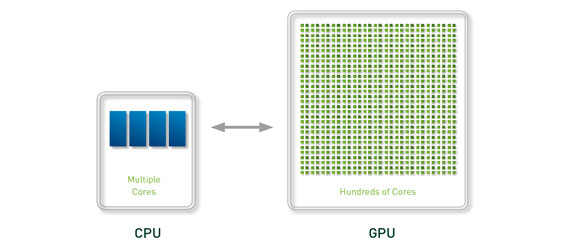
\includegraphics[width=15cm, keepaspectratio]{marco_teorico/cpu_vs_gpu_cores.jpg}
    \caption*{\textbf{Fuente:} \cite{web:gpgpu}}
  \end{figure}
  








  \printbibliography
\end{document}